

\documentclass[tikz,border=12pt]{standalone}

% a plane with varying y coordinate
\newcommand{\plane}[1]{
	(-1.95, #1, 1.35) --
	++(3.6, 0.6, 0.0) --
	++(0.3, -1.8, -2.7) --
	++(-3.6, -0.6, -0.0) --
	cycle}

\newcommand{\nullspacepicture}{
	% bottom part of the row space line
	\draw (0,0,0) -- (0.3,-1.8,1.233);

	% five planes
	\definecolor{y}{rgb}{1,0.761,0.0};
	\draw[fill=y]\plane{-0.2} node[above,left] {Phenomenon};
	%\draw[fill=gray!20]\plane{0.2};
	
	%\draw[] (-0.06,-0.761) circle (0.5pt) node[right];
	
	\draw (-0.06,-0.761,0.0) -- (0,0,0);
	
	\definecolor{g}{rgb}{0.502,0.745,0.388}
	%fill=g
	\draw[fill=g]\plane{0.6} node[above,left] {Experiment};
	
	%\draw[] (0,0) circle (2.5pt) node[right];
	
	\draw (-.094,.562,-.385) -- (0,0,0);
	
	%\draw[fill=gray!20]\plane{1};
	\definecolor{b}{rgb}{0.424,0.604,0.765};
	%fill=b
	\draw[fill=b]\plane{1.4} node[above,left] {Theory};;

	% top part of the row space line
	\draw (-.094,.562,-.385) -- (-0.3,1.8,-1.233);
}
\newcommand{\rangepicture}[1]{
        % axes
	\draw[help lines,->] (-2,0) -- (2,0);
	\draw[help lines,->] (0,-2) -- (0,2);

        % the line and circles
	\draw (1,-2) -- (-1,2);
	
	\draw[fill=g] (0,0) circle (2.5pt) node[right] {};
	\draw[fill=g] (0,0) circle (2.5pt) node[right] {\textbf{lab setting}};
	\draw[fill=y] (0.4,-0.8) circle (2.5pt) node[right] {observations};
	%\draw[fill=red!50] (0.4,-0.8) circle (2.5pt);
	%\draw[fill=gray!50] (-0.2,0.4) circle (2.5pt);
	\draw[fill=b] (-0.4,0.8) circle (2.5pt) node[label={[xshift=1.0cm, yshift=-0.2cm] $hypotheses$}]{};
	\draw[fill=b] (-0.4,0.8) circle (2.5pt) node[left] {};
}


\usepackage{Sweave}
\begin{document}
\Sconcordance{concordance:knowledge_domain_science.tex:knowledge_domain_science.Rnw:%
1 59 1 1 0 31 1}

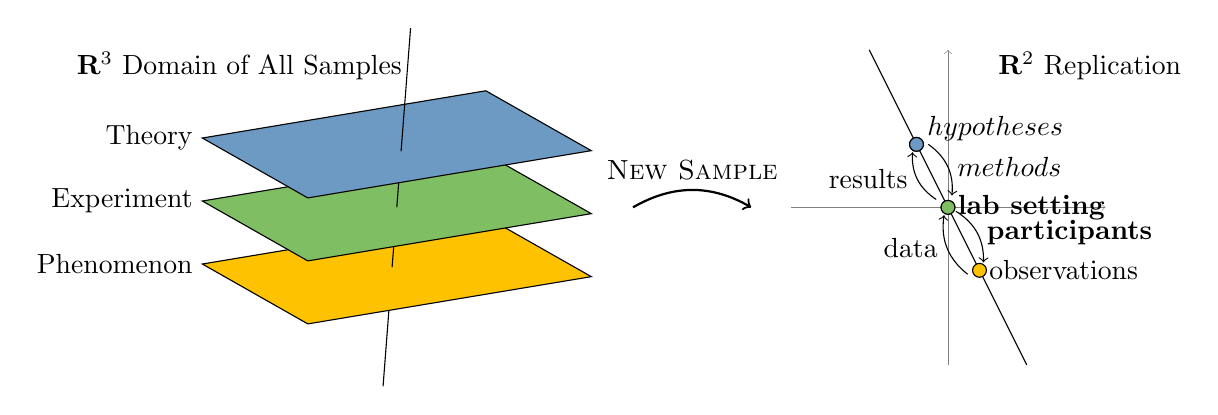
\begin{tikzpicture}
	\nullspacepicture

        % the label
	\node at (-2,1.8) {$\mathbf R^3$ Domain of All Samples};

	% arrow between diagrams
	\path[->] (3,0) edge[thick, bend left] node[above] {\textsc{New Sample}} (4.5,0);




	\begin{scope}[xshift=7cm]
		\rangepicture{}
		\node at (1.8,1.8) {$\mathbf R^2$ Replication};
		% arrow from t to e
	    \path[->] (-0.25,0.8) edge[bend left] node[midway,right] {$methods$} (0.05,0.15);
	    %arrow from e to p
	    \path[->] (0.1,-0.05) edge[bend left] node[midway,right] {\textbf{participants}} (0.45,-0.7);
	    % arrow from e to t
	    \path[->] (-0.15,0.1) edge[bend left] node[above,left] {results} (-0.45,0.7);
	    %arrow from p to e
	    \path[->] (0.25,-0.85) edge[bend left] node[above,left] {data} (-0.05,-0.1);
	\end{scope}
\end{tikzpicture}
\end{document}




